\section{Tính bộ phận công tác}
\subsection{Tính bước của trục vít tải}
\begin{itemize}
    \item Ta chọn vật liệu là Inox 304 vì nó có độ bền cao, khả năng chống ăn mòn tốt phù hợp với môi trường làm việc của máy ép bùn.
    \item Ta sử dụng vít tải quay chậm để vận chuyển vật liệu theo phương nằm ngang. 
    \item Khi trục vít quay thì vật liệu được nâng lên và cả khối vật liệu bị nghiêng đi một góc $\varphi $ như hình dưới, tại đó trọng lượng của vật liệu sẽ cân bằng với lực ma sát của vật liệu với thành máy.
\end{itemize}
\begin{figure}[H]
    \centering
    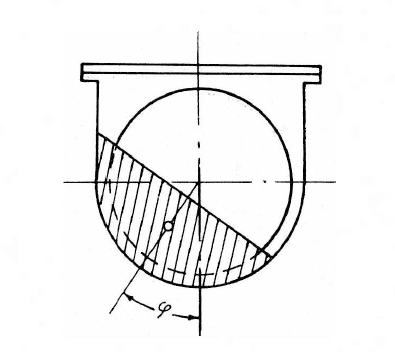
\includegraphics[width=0.5\textwidth]{pictures/vittai1.png}
\end{figure}

\begin{itemize}
    \item Bước của trục vít (hay khoảng cách giữa các cánh vít) đối với vật liệu dạng bột hoặc hạt nhỏ được xác định là:
    \[
        S = (0.7 \div 1)D = 0.8 \cdot 225 = 180 (mm) 
    \]
\end{itemize}
\subsection{Diện tích tiết diện ngang do vật liệu chiếm trong thành máy}
\[
    F = \frac{\pi\cdot D^2}{4}\mu \cdot K = \frac{\pi\cdot 0.225^2}{4}\cdot 0.35\cdot 1 = 0.0139 (m^2)
\]
Trong đó: 
\begin{itemize}
    \item D = 225 mm, là đường kính của vít tải
    \item $\mu$ là hệ số chứa vật liệu trong thành máy. Với vật liệu dạng bột ta chọn $\mu = 0.35$
    \item K là hệ số chỉ sự giảm tiết diện do góc nghiêng đặt vít tải. Với góc nghiêng bằng $0^{\circ}$ ta chọn $K = 1$
\end{itemize}
\subsection{Vận tốc chuyển vật liệu dọc theo trục vít}
\[
    v = \frac{S\cdot n_{ct}}{60} = \frac{0.18\cdot 118.85}{60} = 0.356 (m/s)
\]
Trong đó: 
\begin{itemize}
    \item $S = 180 mm$: bước của vít tải
    \item $n_{ct} = 118.85$ vòng/phút: số vòng quay của trục vít tải
\end{itemize}
\subsection{Xác định năng xuất máy}
\[
    Q = 3600F\cdot v\cdot \rho = 3600\cdot 0.0139\cdot 0.356\cdot 1000 = 17814.24 (kg/h)
\]
Trong đó:
\begin{itemize}
    \item $F = 13916.27 mm^2$: diện tích ngang do vật liệu chiếm trong thành máy
    \item $v = 0.356$ m/s: vận tốc chuyển vật liệu dọc theo trục vít
    \item $\rho = 1000$ kg/m$^3$: khối lượng riêng của bùn
\end{itemize}

